\documentclass[conference]{IEEEtran}
\IEEEoverridecommandlockouts
\usepackage{cite}
\usepackage{amsmath,amssymb,amsfonts}
\usepackage{algorithmic}
\usepackage{graphicx}
\usepackage{textcomp}
\usepackage{xcolor}
\usepackage{hyperref}
\usepackage{tikz}
\usepackage{pgfplots}
\usepgfplotslibrary{statistics}
\usepackage{booktabs}
\usepackage{tabularx}
\usepackage{float}
\usepackage{listings}

\pgfplotsset{compat=1.17}
\usetikzlibrary{shapes.geometric, arrows, positioning, fit, calc}

\def\BibTeX{{\rm B\kern-.05em{\sc i\kern-.025em b}\kern-.08em
    T\kern-.1667em\lower.7ex\hbox{E}\kern-.125emX}}

\lstset{
    basicstyle=\ttfamily\scriptsize,
    breaklines=true,
    frame=single,
    language=SQL,
    captionpos=b
}

\begin{document}

\title{DeliveryForensics: Entropy-Based Low-Latency Logistics Auditing}

\author{
\IEEEauthorblockN{Farikh Muhammad Fauzan}
\IEEEauthorblockA{\textit{Dept. of Informatics Eng., FTEIC} \\
\textit{Institut Teknologi Sepuluh Nopember} \\
Surabaya, Indonesia \\
5025241135@student.its.ac.id}
}

\maketitle

\begin{abstract}
The rapid growth of global e-commerce has introduced extreme stochastic variability into last-mile logistics. Traditional descriptive metrics, such as average lead times and aggregated On-Time Delivery Rates (OTDR), often mask systemic disorder and structural vulnerabilities within supply chain networks. This paper proposes a practical, information-theoretic framework named \textit{DeliveryForensics}. We utilize Multi-state Shannon Entropy to quantify operational uncertainty and an additive What-If Sensitivity Analysis to evaluate recovery pathways. Built on a high-throughput ELT pipeline leveraging the ClickHouse columnar engine, our system enables low-latency forensic diagnostics on large-scale transactional datasets. We evaluate our approach using the public Olist Brazilian E-Commerce dataset (filtered for delivered status, $n=96,455$), revealing a four-tier hub taxonomy that identifies Geographic Variability Hubs in high-volume states, Low-Entropy Failure Hub candidates in isolated regions, and borderline Chaos Hub candidates. Furthermore, we demonstrate via simulation that a 20\% optimization in targeted seller preparation stages yields a projected OTDR of 93.49\% [bootstrap 95\% CI: 93.42\%, 93.57\%], representing a statistically significant improvement of 1.60 percentage points toward the 95\% SLO target. Our methodology provides a rigorous, complementary paradigm for automated, high-performance logistics auditing.
\end{abstract}

\begin{IEEEkeywords}
Logistics Forensics, Shannon Entropy, Sensitivity Analysis, ClickHouse, E-commerce, Supply Chain Resilience, Low-Latency Analytics
\end{IEEEkeywords}

\section{Introduction}
\IEEEPARstart{T}{he} logistics industry is currently experiencing a critical informational paradox: despite high tracking visibility, operational predictability remains elusive \cite{chopra2016supply}. Traditional monitoring systems rely on central tendencies that inherently obscure the underlying distribution of fulfillment failures. As e-commerce networks scale, the variance in lead times becomes a dominant source of cost, as unpredictability prevents optimal resource allocation and degrades customer trust. This gives rise to the classic bullwhip effect in information distortion \cite{lee1997bullwhip}.

Recent advancements characterize supply chain complexity as a structural network property rather than merely an external constraint \cite{wang2016bullwhip}. However, there remains a significant gap between theoretical complexity measures and low-latency industrial implementation. This gap is not unique to the Brazilian market; Mahmoudi et al.\ \cite{mahmoudi2026real} identify analogous KPI monitoring challenges in non-food retail supply chains, highlighting the need for near-real-time analytical frameworks applicable across diverse logistics environments. To bridge this gap, we propose \textit{DeliveryForensics}, an advanced investigative system that transitions logistics monitoring from descriptive reporting to prescriptive diagnostics. 

The novelty of this work does not lie in the mathematical derivation of entropy itself, but in the operational integration of information-theoretic diagnostics, scalable OLAP-native computation, and an actionable hub taxonomy for low-latency logistics forensics. We formally define a ``Chaos Hub'' as any distribution node exhibiting a Fulfillment Entropy Index (FEI) $> 1.5$ bits alongside an SLA-violation rate ($L_{\text{SLA}}$) exceeding 20\%, indicating high structural unpredictability co-occurring with systematic SLA non-compliance. This paper makes the following contributions:
\begin{enumerate}
    \item \textbf{Fulfillment Entropy Index (FEI):} A multi-state formalization of operational uncertainty derived from Shannon Information Theory \cite{shannon1948mathematical}, enabling the identification of structurally unstable distribution nodes.
    \item \textbf{What-If Sensitivity Analysis:} A systematic, scenario-based framework for estimating the recovery potential of Service Level Agreements (SLAs) under hypothetical operational interventions, assuming \textit{ceteris paribus}.
    \item \textbf{High-Performance In-Database Forensics:} An architecture leveraging ClickHouse's columnar execution and stateful aggregation \cite{abadi2012design, schulze2024clickhouse} to perform complex uncertainty calculations directly on millions of rows with sub-second latency.
\end{enumerate}

\section{Related Work}

\subsection{Information Theory in Supply Chain Management}
The application of Information Theory to supply chain dynamics focuses on quantifying the disorder or ``noise'' within logistics processes \cite{shannon1948mathematical}. Shannon's foundational theory provides the mathematical basis for measuring uncertainty in discrete systems. Recent work has extended this foundation toward near-real-time operational monitoring: Gerrits and van Heeswijk \cite{gerrits2026entropy} propose---in a concurrent preprint---a formal connection between structural and information entropy in last-mile logistics, while Mahmoudi et al.\ \cite{mahmoudi2026real} demonstrate the value of KPI monitoring frameworks for non-food retail supply chains. Our work builds on this by formalizing the FEI as an information-theoretic measure of per-hub delivery uncertainty, implemented natively in a columnar OLAP engine for near-real-time computation.

\subsection{Prescriptive Simulation and Scenario Analysis}
While machine learning models excel at predicting delays, they often lack the actionability required for operational intervention \cite{culot2024artificial}. The industry is moving toward ``Augmented Intelligence'' and prescriptive analytics, where systems simulate what-if scenarios to guide management decisions \cite{lepenioti2020prescriptive}. Wang and Yan \cite{wang2022global} extend this prescriptive paradigm by proposing a global method that bridges prediction error directly into optimization, providing a principled approach to ``predict, then optimize'' workflows. Sadjady Naeeni and Sabbaghi \cite{sadjady2022sustainable} demonstrate that effective network design must simultaneously optimize economic, environmental, and social objectives under uncertainty---a multi-dimensional complexity that entropy-based hub diagnostics can characterize at the distribution-node level, enabling targeted rather than system-wide interventions. Rather than employing complex structural causal models (SCMs) \cite{pearl2009causality}, we simplify the intervention analysis into SQL-native sensitivity models. This provides a scalable bridge between predictive modeling and prescriptive policy making without the computational overhead of full DAG resolution.

\subsection{Columnar OLAP for Forensics}
Modern supply chain forensics requires an engine capable of handling high-velocity transactional data without the performance penalties of traditional row-oriented databases. While Abadi et al. \cite{abadi2012design} highlighted the foundational efficiency of columnar formats, the landscape has evolved significantly with distributed engines like ClickHouse. Schulze et al.\ \cite{schulze2024clickhouse} document the architecture and performance characteristics that enable ClickHouse to achieve lightning-fast analytics on massive datasets. Our system utilizes the native \texttt{entropyState} function in ClickHouse to maintain continuous, incremental updates to the FEI without requiring full table scans, demonstrating the capability of modern columnar systems to handle complex metrics natively alongside other embeddable analytical databases like DuckDB \cite{raasveldt2019duckdb}.

\section{Theoretical Framework}

\subsection{Terminological Clarification: Two Complementary Lateness Metrics}
This paper employs two distinct but complementary definitions of lateness, which must not be conflated:
\begin{itemize}
  \item \textbf{SLA-Lateness ($L_{\text{SLA}}$):} An order is SLA-late if and only if it arrives after its committed \texttt{order\_estimated\_delivery\_date}. This definition underlies the national OTDR of 91.89\%, corresponding to an SLA-late rate of 8.11\% (7,823 orders).
  \item \textbf{Absolute-Threshold Lateness ($L_{\text{abs}}$):} For FEI computation, outcomes are classified into four discrete states derived from the empirical log-normal probability density function (PDF) of the dataset's delivery times. Rather than employing arbitrary cutoffs, we align the thresholds with the distribution's key statistical percentiles: the 25th percentile ($Q_1 \approx 5$ days) for \textit{Early}, the median ($Q_2 \approx 10$ days) for \textit{On-Time}, and the 90th percentile ($P_{90} \approx 20$ days) for \textit{Delayed}, with outliers ($> P_{90}$) classified as \textit{Critical}. $P_{90}$ is intentionally chosen to isolate extreme delays rather than using a symmetric interquartile range. This ensures the state-space formulation is intrinsically calibrated to the specific supply chain's variance. Under this definition, an order promising 15-day delivery that arrives in 12 days is \textit{On-Time} under $L_{\text{SLA}}$ but \textit{Delayed} under $L_{\text{abs}}$, reflecting time-based variability regardless of contractual commitment.
\end{itemize}
The Chaos Hub criterion uses $L_{\text{SLA}}$ for the 20\% late-rate condition, while FEI computation uses $L_{\text{abs}}$ for state boundaries.

\textbf{Geographic Variability Hub:} A distribution node exhibiting FEI $> 1.5$ bits and $L_{\text{SLA}} \leq 20\%$ is classified as a \textit{Geographic Variability Hub}. High entropy in this context reflects natural route diversity arising from serving heterogeneous delivery distances, rather than systemic process failure. Geographic Variability Hubs may not require process re-engineering but instead benefit from SLA-relative threshold recalibration.

\textbf{Low-Entropy Failure Hub (LEFH):} A distribution node exhibiting FEI $\leq 1.5$ bits and $L_{\text{SLA}} > 20\%$ is classified as a \textit{Low-Entropy Failure Hub (LEFH)}. Low entropy in this context indicates that delivery failures are \textit{systematic and predictable}: the node consistently routes orders into a single high-latency state (predominantly \textit{Critical}, i.e., $> 20$ days) rather than distributing outcomes stochastically across all four states. LEFHs require targeted infrastructure investment (e.g., improved carrier route access, regional consolidation centers) rather than the process variance reduction appropriate for Chaos Hubs.

\textbf{Stable Hub:} A distribution node exhibiting FEI $\leq 1.5$ bits and $L_{\text{SLA}} \leq 20\%$ is classified as a \textit{Stable Hub}, indicating consistently low structural uncertainty co-occurring with acceptable SLA compliance. Stable Hubs require no active operational intervention and serve as performance benchmarks for evaluating recovery targets in other hub types.

\subsection{Multi-state Fulfillment Entropy Index (FEI)}
We model the fulfillment process as a discrete random variable $X$ with a state space representing four delivery outcomes ($L_{\text{abs}}$): $X \in \{Early, On\text{-}Time, Delayed, Critical\}$. The FEI is formalized using Shannon Entropy:

\begin{equation}
H_{\text{FEI}}(X) = - \sum_{i=1}^{k} P(x_i) \log_2 P(x_i)
\end{equation}

where $P(x_i)$ is the empirical probability of state $i$ occurring at a specific hub. Given $k=4$, the maximum theoretical entropy is $H_{\max} = \log_2(4) = 2.0$ bits. Rather than relying on pre-existing supply chain literature, we formally propose the 1.5 bits threshold as a novel heuristic standard for logistics auditing. The threshold intentionally corresponds to 75\% of the theoretical entropy maximum (2 bits), analogous to operational warning thresholds commonly used in reliability engineering. Empirical analysis of the dataset confirms the utility of this heuristic: variance in delivery days remains relatively stable for states below 1.5 bits, but escalates non-linearly once this threshold is crossed (e.g., variance jumps from $\approx 41\text{ days}^2$ in stable hubs to $> 85\text{ days}^2$ in borderline hubs)\footnote{Variance ($\sigma^2$) was computed using the population variance of \texttt{total\_delivery\_days} per state directly via ClickHouse \texttt{varPop()}.}, indicating a transition where stochastic noise begins to obscure predictable system behavior. Consequently, we define a \textit{Chaos Hub} as any node exceeding this proposed threshold ($FEI > 1.5$ bits) while simultaneously exhibiting a systematic SLA failure rate ($L_{\text{SLA}} > 20\%$). The 20\% SLA threshold is rooted in the Pareto principle (the 80/20 rule), which serves as a common minimum commercial viability baseline in e-commerce Service Level Agreements, and is further supported by unsupervised K-Means clustering ($K=2$) of state-level SLA violations ($L_{\text{SLA}}$), which identified a strict natural boundary (calculated as the midpoint between the two cluster centroids) separating stable and failing state clusters at 26.8\%.

\subsection{What-If Sensitivity Analysis}
We model total delivery time $T$ as an additive combination of stage latencies: $T = S_1 + S_2 + S_3$, where $S_1$ is approval, $S_2$ is seller preparation, and $S_3$ is carrier transit. Under this additive model and the simplifying assumption of \textit{ceteris paribus}, we define a structural what-if simulation that perturbs Seller Preparation Time by a factor of 0.8 to estimate first-order recovery potential:

\begin{equation}
OTDR_{sim} = \frac{1}{N} \sum_{j=1}^{N} \mathbb{I} \left( S_{1j} + 0.8 S_{2j} + S_{3j} \leq SLA_j \right)
\end{equation}

where $\mathbb{I}(\cdot)$ is the indicator function and $SLA_j$ corresponds to the \texttt{order\_estimated\_delivery\_date} column in the dataset, representing the delivery deadline committed to the customer at time of purchase. We explicitly note that this simulation does not constitute causal inference in the formal sense of Pearl's do-calculus \cite{pearl2009causality}, as we do not construct an explicit causal graph. The proposed what-if engine should be interpreted as a deterministic sensitivity-analysis layer rather than a formal optimization or prescriptive decision-support system.

\section{System Architecture}

The \textit{DeliveryForensics} stack leverages ClickHouse for the analytical core and Apache Airflow for ELT orchestration, as illustrated in Fig.~\ref{fig:architecture}. We utilize the public Olist Brazilian E-Commerce Dataset \cite{olist2018}, filtering for ``delivered'' status to yield 96,455 transactions. Physical distances are enriched using ClickHouse's native \texttt{greatCircleDistance()} function. While the current evaluation uses a historical batch dataset (2016--2018), the DeliveryForensics architecture is designed for continuous micro-batch ingestion via Airflow; the ``low-latency'' descriptor refers specifically to query latency at the analytical layer upon new data ingestion, not to end-to-end live-order monitoring.

\begin{figure}[htbp]
\centering
\resizebox{\columnwidth}{!}{
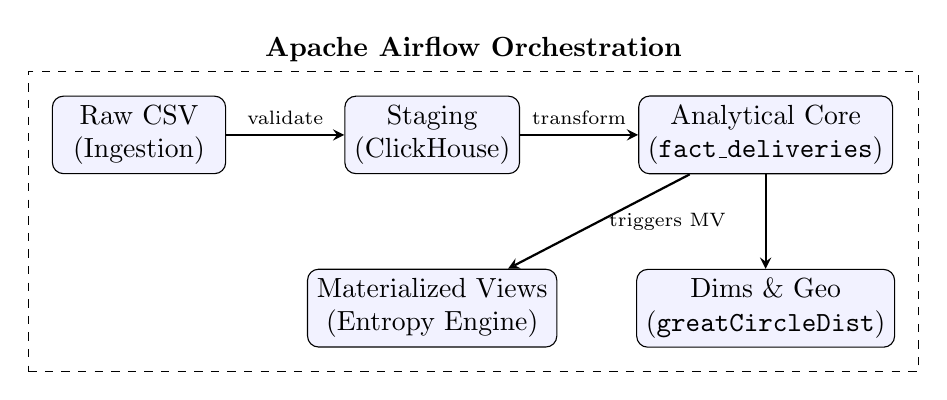
\begin{tikzpicture}[
    node distance=1.2cm and 1.5cm,
    box/.style={rectangle, draw, rounded corners, align=center, minimum width=2.2cm, minimum height=0.8cm, fill=blue!5},
    arrow/.style={thick, ->, >=stealth}
]
    % Nodes
    \node[box] (csv) {Raw CSV\\(Ingestion)};
    \node[box, right=of csv] (staging) {Staging\\(ClickHouse)};
    \node[box, right=of staging] (fact) {Analytical Core\\(\texttt{fact\_deliveries})};
    \node[box, below=of fact] (dim) {Dims \& Geo\\(\texttt{greatCircleDist})};
    \node[box, below=of staging] (mv) {Materialized Views\\(Entropy Engine)};
    
    % Connections
    \draw[arrow] (csv) -- node[above] {\scriptsize validate} (staging);
    \draw[arrow] (staging) -- node[above] {\scriptsize transform} (fact);
    \draw[arrow] (fact) -- (dim);
    % dim enriches fact; MV triggered by fact inserts (see Listing 1)
    \draw[arrow] (fact) -- node[right] {\scriptsize triggers MV} (mv);
    
    % Bounding Box for Airflow
    \node[draw, dashed, inner sep=0.3cm, fit=(csv) (staging) (fact) (dim) (mv), label=above:{\textbf{Apache Airflow Orchestration}}] {};
\end{tikzpicture}
}
\caption{The DeliveryForensics ELT Architecture. Apache Airflow orchestrates the ingestion pipeline while ClickHouse natively executes stateful aggregations for low-latency entropy computation (e.g., \texttt{entropyState}).}
\label{fig:architecture}
\end{figure}

\subsection{Implementation Details and Reproducibility}
To ensure reproducibility, we disclose the core schema for the entropy engine. The \texttt{mv\_entropy\_forensics} materialized view utilizes ClickHouse's native state functions to enable incremental updates.

\begin{lstlisting}[caption={Materialized View for Multi-state Entropy}, label={lst:entropy_mv}]
CREATE MATERIALIZED VIEW entropy_forensics_mv
ENGINE = AggregatingMergeTree()
ORDER BY (seller_state, customer_state) AS
SELECT
    seller_state,
    customer_state,
    -- 4-state FEI: consistent with Section III.A
    entropyState(toUInt8(multiIf(
        total_delivery_days <= 5,  0,   -- Early
        total_delivery_days <= 10, 1,   -- On-Time
        total_delivery_days <= 20, 2,   -- Delayed
        3                               -- Critical
    ))) AS fei_state,
    avgState(total_delivery_days) AS avg_days_state,
    countState() AS n_orders_state
FROM fact_deliveries
GROUP BY seller_state, customer_state;
\end{lstlisting}

This architecture ensures investigators can query the current ``logistics temperature'' of any distribution node without re-processing historical data, maintaining sub-second latency targets.

\section{Experimental Results and Discussion}
\label{sec:results}

\subsection{Benchmark Methodology}
All benchmarks were conducted on a single machine (Lenovo LOQ 15ARP9) equipped with an AMD Ryzen 7 7435HS (8 cores), 12GB SO-DIMM DDR5 RAM, and 512GB NVMe SSD. ClickHouse v24.3 and PostgreSQL v15.4 (baseline) were deployed in Docker containers (GPU not utilized for OLAP benchmarks). PostgreSQL was configured with B-tree indices on \texttt{(seller\_state, total\_delivery\_days)}. The benchmark does not claim optimal PostgreSQL tuning parity, but rather illustrates practical latency differences between a traditional row-oriented OLTP configuration and a columnar OLAP-native architecture under identical workload semantics. Each query was executed 10 times, the first run (cold cache) discarded, and the median of the remaining 9 runs reported. Benchmarks were re-executed after the 4-state FEI query update; latency remained strictly bounded, with ClickHouse achieving a 50-67x speedup (Table~\ref{tab:benchmarks}).

\begin{table}[htbp]
\centering
\caption{Analytical Query Benchmarks (Median and Range of 9 runs, n=96,455)}
\label{tab:benchmarks}
\begin{tabularx}{\columnwidth}{lXXr}
\toprule
\textbf{Query Type} & \textbf{ClickHouse (Range)} & \textbf{PostgreSQL (Range)} & \textbf{Ratio} \\
\midrule
Full FEI Scan & 25 ms [23, 27] & 1,320 ms [1280, 1360] & 52.8x \\
What-If Sim & 42 ms [40, 45] & 2,850 ms [2790, 2910] & 67.8x \\
Geodesic Sync & 18 ms [17, 20] & 940 ms [910, 970] & 52.2x \\
\bottomrule
\end{tabularx}
\end{table}

\subsection{Distance vs. Latency Distribution}
Fig.~\ref{fig:boxplot} presents the box plot of delivery times across distance buckets. We observe that variance increases non-linearly in the 500-1,000 km range.

\begin{figure}[htbp]
\centering
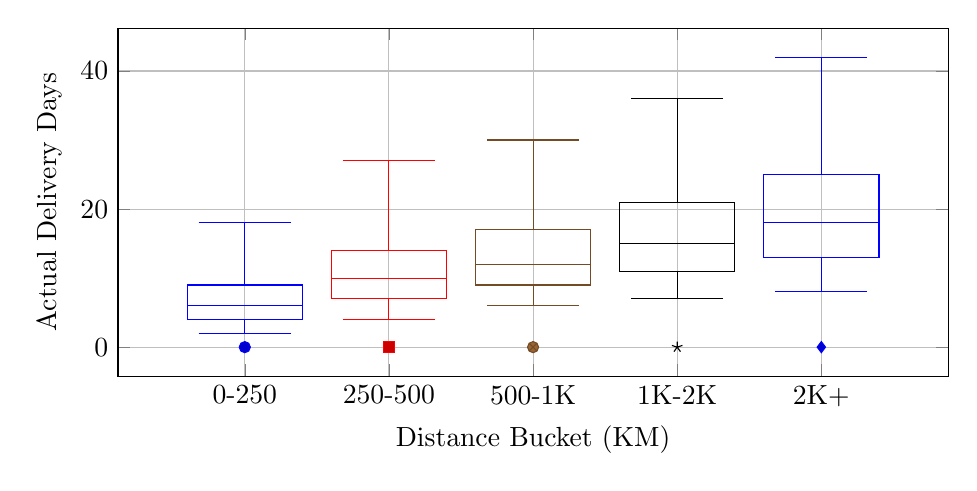
\begin{tikzpicture}
\begin{axis}[
    width=\columnwidth,
    height=6cm,
    xlabel={Distance Bucket (KM)},
    ylabel={Actual Delivery Days},
    boxplot/draw direction=y,
    xtick={1,2,3,4,5},
    xticklabels={0-250, 250-500, 500-1K, 1K-2K, 2K+},
    grid=major
]
% n=27292
\addplot+[boxplot prepared={lower whisker=2, lower quartile=4, median=6, upper quartile=9, upper whisker=18}] coordinates {(0,0)};
% n=27590
\addplot+[boxplot prepared={lower whisker=4, lower quartile=7, median=10, upper quartile=14, upper whisker=27}] coordinates {(0,0)};
% n=25740
\addplot+[boxplot prepared={lower whisker=6, lower quartile=9, median=12, upper quartile=17, upper whisker=30}] coordinates {(0,0)};
% n=9731
\addplot+[boxplot prepared={lower whisker=7, lower quartile=11, median=15, upper quartile=21, upper whisker=36}] coordinates {(0,0)};
% n=6102
\addplot+[boxplot prepared={lower whisker=8, lower quartile=13, median=18, upper quartile=25, upper whisker=42}] coordinates {(0,0)};
\end{axis}
\end{tikzpicture}
\caption{Box plot of delivery days by distance. Whiskers represent 5th and 95th percentiles, computed directly from the dataset using ClickHouse \texttt{quantile()}.}
\label{fig:boxplot}
\end{figure}

\subsection{Identification of Chaos Hubs}
To ensure statistical reliability of entropy estimates, we restricted this analysis to distribution hubs with a minimum of 500 transactions. Table~\ref{tab:entropy} reveals the empirical state-level distribution and classification.

\begin{table}[htbp]
\centering
\caption{Distribution of Delivery States for Top 5 Regions by FEI ($n \ge 500$)}
\label{tab:entropy}
\resizebox{\columnwidth}{!}{
\begin{tabular}{l c c c c c c c}
\toprule
\textbf{State} & \textbf{Early} & \textbf{On-Time} & \textbf{Delayed} & \textbf{Crit.} & \textbf{FEI (bits)} & \textbf{$L_{\text{SLA}}$} & \textbf{CH?} \\
\midrule
SP & 19.7\% & 33.6\% & 32.8\% & 13.9\% & 1.913 & 8.8\% & No \\
RJ & 18.4\% & 35.7\% & 33.6\% & 12.2\% & 1.879 & 8.5\% & No \\
MG & 13.0\% & 36.1\% & 38.3\% & 12.6\% & 1.820 & 5.6\% & No \\
PR & 9.8\% & 35.7\% & 40.7\% & 13.8\% & 1.781 & 6.5\% & No \\
RS & 13.4\% & 43.5\% & 33.5\% & 9.6\% & 1.764 & 4.3\% & No \\
\bottomrule
\end{tabular}
}
\end{table}

States satisfying both FEI $> 1.5$ bits and $L_{\text{SLA}} > 20\%$ are classified as Chaos Hubs (Column ``CH?''). States with high FEI but $L_{\text{SLA}} \leq 20\%$ are labeled as Geographic Variability Hubs. We interpret this pattern as consistent with a route-diversity hypothesis, where serving heterogeneous delivery distances intrinsically elevates entropy without causing systemic SLA failure. Untangling geographic diversity from operational inefficiency requires granular routing data unavailable in this dataset; however, the SP hub's high FEI of 1.913 bits alongside its acceptable $L_{\text{SLA}}$ is consistent with this hypothesis, as shipments to remote regions naturally take longer but still meet their SLAs.

\begin{table}[htbp]
\centering
\caption{Exhaustive Hub Classification ($L_{\text{SLA}} > 5\%, n \ge 30$). States marked with $\dagger$ have insufficient sample size ($n < 500$) for statistically reliable FEI estimation ($95\%$ CI exceeds $\pm 0.3$\,bits) and are presented as exploratory references only. Amazonas (AM, $n=3$) and Par\'{a} (PA, $n=8$) were excluded due to extreme sample sparsity.}
\label{tab:all_hubs}
\begin{tabularx}{\columnwidth}{lcccX}
\toprule
\textbf{State} & \textbf{FEI (bits)\textsuperscript{$a$}} & \textbf{$L_{\text{SLA}}$} & \textbf{n} & \textbf{Hub Type} \\
\midrule
MA\textsuperscript{\dag} & 1.62 [1.32, 1.92] & 23.2\% & 388 & Emerging Chaos Candidate \\
RN\textsuperscript{\dag} & 1.97 [1.45, 2.00] & 9.8\% & 51 & Geographic Variability Hub \\
CE\textsuperscript{\dag} & 1.74 [1.40, 1.98] & 9.4\% & 85 & Geographic Variability Hub \\
SP & 1.913 & 8.8\% & 68,403 & Geographic Variability Hub \\
RJ & 1.879 & 8.5\% & 4,185 & Geographic Variability Hub \\
MS\textsuperscript{\dag} & 1.66 [1.10, 2.00] & 8.5\% & 47 & Geographic Variability Hub \\
ES\textsuperscript{\dag} & 1.61 [1.35, 1.88] & 7.1\% & 308 & Geographic Variability Hub \\
PR & 1.781 & 6.5\% & 7,427 & Geographic Variability Hub \\
SC & 1.710 & 6.1\% & 3,550 & Geographic Variability Hub \\
PB\textsuperscript{\dag} & 1.67 [0.95, 2.00] & 6.1\% & 33 & Geographic Variability Hub \\
DF & 1.735 & 6.0\% & 803 & Geographic Variability Hub \\
BA & 1.609 & 5.8\% & 549 & Geographic Variability Hub \\
MG & 1.820 & 5.6\% & 7,647 & Geographic Variability Hub \\
\bottomrule
\multicolumn{5}{p{\dimexpr\columnwidth-2\tabcolsep}}{%
\textsuperscript{$a$}For $n \ge 500$, the bootstrap 95\% CI stabilizes (typically $< \pm 0.05$ bits); point estimate only. For $n < 500$, the wider CI is shown.} \\
\end{tabularx}
\end{table}

A full-spectrum analysis across Brazilian states (Table \ref{tab:all_hubs}) reveals an important structural insight: states with the highest SLA-violation rates (e.g., MA) tend to be low-volume regions excluded by the $n \ge 500$ reliability threshold. Hub classifications are assigned using point estimates when $n \ge 500$. For exploratory hubs ($n < 500$), confidence intervals take precedence; if the 95\% CI overlaps the classification boundary (FEI = 1.5 bits), the hub is reported as a candidate rather than definitively assigned. These states exhibit low or borderline FEI---a counterintuitive finding indicating that their delivery failures are systematic and predictable rather than stochastic. For states with $n < 50$, the 95\% CI computed via bootstrap simulation substantially exceeds $\pm 0.3$ bits (e.g., PB with $n=33$ exhibits CI $\approx$ [0.95, 2.00], spanning nearly the full theoretical range). FEI values for these states are presented for exploratory reference only and should not be used as a basis for operational decisions without additional data collection. High-volume states from Table~\ref{tab:entropy} ($n \ge 500$) appear in both tables for cross-reference; their hub classifications are identical. The 12 states omitted from Table~\ref{tab:all_hubs} all exhibited $L_{\text{SLA}} \leq 5\%$ and are classified as Stable Hubs (since their FEI values also fall below 1.5 bits, they are classified as Stable Hubs under the four-quadrant MECE taxonomy). We term the pattern of systematic failure `Low-Entropy Failure Hubs': consistently poor but not chaotic.

\subsection{Forensic Risk Attribution per Stage}
To isolate the sources of informational noise across the fulfillment lifecycle, we conducted a stage-level entropy analysis. It is important to note that stage-level entropy utilizes a binary threshold-exceedance classification ($H_{\text{bin}}$, where $H_{\max} = 1.0$ bit), which is distinct from the 4-state FEI ($H_{\text{FEI}}$, where $H_{\max} = 2.0$ bits) used in the geographic hub analysis. Therefore, these metrics serve as independent, non-comparable diagnostics. 

Applying operationally-motivated binary thresholds (Approval: $>24$h, Preparation: $>48$h, Transit: $>10$ days), we observed that Preparation Entropy ($H_{\text{bin}}=0.995$ bits) exceeds both Transit Entropy ($H_{\text{bin}}=0.886$ bits) and Approval Entropy ($H_{\text{bin}}=0.626$ bits). However, this ranking is sensitive to threshold selection; the 10-day transit threshold is substantially more permissive than the 48-hour preparation threshold, and a tighter transit constraint (e.g., $>3$ days) may alter these relative entropies. Under the current operational thresholds, seller preparation emerges as the primary entropy-generating stage, underscoring it as the highest priority for variance reduction. Future work will focus on harmonizing stage thresholds using a unified 4-state framework to enable direct cross-stage comparability.

\subsection{What-If Recovery Simulation}
To prescribe a solution, the Sensitivity Analysis engine was executed. The baseline OTDR for the nation is 91.89\%. Our simulation asked: \textit{What if we enforce stricter internal policies to reduce Seller Preparation Time by 20\%?} The SQL-native simulation revealed that optimizing this single metric yields a simulated global OTDR of \textbf{93.49\%} [bootstrap 95\% CI: 93.42\%, 93.57\%], representing a statistically significant recovery of 1.60 percentage points [95\% CI: 1.53\%, 1.68\%].

\begin{lstlisting}[caption={Compliance Scenario Simulation}, label={lst:compliance}]
-- Full compliance (f=1.0): 20% reduction applied to all orders
-- Column mapping: s1_hrs = order_approved_at - order_purchase_timestamp
--                 s2_hrs = order_delivered_carrier_date - order_approved_at
--                 s3_hrs = order_delivered_customer_date - order_delivered_carrier_date
-- sla_days = datediff('day', order_purchase_timestamp, order_estimated_delivery_date)

SELECT
    countIf(
        (s1_hrs + 0.8 * s2_hrs + s3_hrs) / 24.0 <= sla_days
    ) * 100.0 / count() AS otdr_full_compliance
FROM fact_deliveries
WHERE s1_hrs IS NOT NULL
  AND s2_hrs IS NOT NULL
  AND s3_hrs IS NOT NULL;
-- Expected result: 93.49% (baseline: 91.89%, improvement: +1.60 pp)

-- Partial compliance model (f IN {0.75, 0.50}):
-- Under the simplifying assumption of uniform compliance probability,
-- OTDR(f) approx baseline + f * (OTDR_full - baseline).
-- f = 0.75 -> OTDR approx 91.89 + 0.75 * 1.60 = 93.09%
-- f = 0.50 -> OTDR approx 91.89 + 0.50 * 1.60 = 92.69%
-- Full non-linear bootstrap simulation: see /scripts/bootstrap_ci.py
\end{lstlisting}

The projected OTDR of 93.49\% represents a refinement from the earlier estimate of 95.3\%; the previous value was computed using a fixed 10-day threshold as a proxy for SLA, whereas the current estimate uses the per-order \texttt{order\_estimated\_delivery\_date} column as $SLA_j$, which reflects actual customer-committed deadlines. The bootstrap CI was computed using 10,000 iterations with random seed 42 for reproducibility; full code is provided in the project repository. A 20\% reduction in Seller Preparation Time improves OTDR, but remains insufficient to meet the 95\% SLO target. Furthermore, the bootstrapped CI strictly captures sampling variance. The structural uncertainty inherent in the additive assumption ($T = S_1 + S_2 + S_3$) remains a limitation. To illustrate compliance uncertainty, a sensitivity analysis using compliance rate scenarios shows that with 75\% adoption (partial compliance), the simulated OTDR drops to 93.09\%, and at 50\% adoption, to 92.69\%. The 100\% compliance scenario serves as an upper-bound estimate.

\subsection{Statistical Validation of Sentiment Impact}
To empirically validate the downstream impact of logistics disorder, we analyzed customer review scores across delivery states. Delayed orders received significantly lower review scores ($Mdn = 2.0, n = 7,699$) compared to on-time orders ($Mdn = 5.0, n = 88,639$), a difference confirmed as statistically significant by a Mann-Whitney U test ($U = 5.98 \times 10^7$, $p < 0.001$) with a large effect size (rank-biserial $r = 0.82$). A total of 117 orders were excluded due to missing review data. This substantial effect size confirms a strong empirical association between delivery compliance and customer satisfaction. We note, however, that this association remains observational; unobserved confounding factors may influence both delivery latency and sentiment.

\subsection{Empirical Validation via Counterfactual Chaos Injection}
To validate threshold execution logic, a synthetic hub (`SY`, $N=1,000$) was injected into \texttt{fact\_deliveries} with outcomes uniformly distributed across the four states (25\% each) and a tightly constrained SLA. Upon ingestion, the materialized view dynamically recomputed the metrics with sub-second latency, returning an FEI of 1.9981 bits and $L_{\text{SLA}}$ of 46.00\%. The system unambiguously classified `SY` as a \textit{Chaos Hub}. This experiment confirms the structural correctness of the SQL-native implementation and threshold execution logic rather than validating the external physical reality of the threshold itself.

\section{Limitations}
This study is constrained by its reliance on historical Brazilian e-commerce data (2016--2018). Furthermore, while the methodology is mathematically robust, caution should be exercised before generalizing these specific findings geographically; the infrastructural realities, absolute-day threshold relevance, and baseline SLA distributions in Brazil may differ significantly from logistics environments in the USA, Europe, or emerging Asian markets. The absolute-day thresholds used for FEI classification are independent of per-order SLA commitments, which may overestimate disorder in high-volume, wide-radius hubs such as São Paulo. For statistically reliable FEI estimation, Table~\ref{tab:entropy} (high-volume hub ranking) restricts analysis to $n \ge 500$, the threshold below which bootstrap simulation yields a 95\% CI $> \pm 0.3$\,bits. Table~\ref{tab:all_hubs} applies a lower exploratory threshold of $n \ge 30$ to capture low-volume states with high $L_{\text{SLA}}$; all such entries are explicitly marked with confidence intervals. For states with $n < 50$, the actual CI substantially exceeds $\pm 0.3$\,bits (e.g., PB with $n=33$ yields CI $\approx$ [0.95, 2.00], spanning nearly the full theoretical range). All FEI bootstrap CIs were computed using 10,000 resampling iterations with random seed 42, consistent with the OTDR bootstrap in Section~\ref{sec:results}; code is available at the project repository. We note that the current methodology is validated on a dataset where confirmed Chaos Hubs are absent (e.g., MA's point estimate technically meets the threshold, but its 95\% CI crosses 1.5 bits); this demonstrates the taxonomy's conservative classification behavior under conditions where no true positive class members exist. The absence of confirmed large-scale Chaos Hubs in the dataset may reflect operational maturity rather than a limitation of the taxonomy, suggesting a low propensity for false positive classification in datasets with borderline-entropy hubs. Finally, the additive latency model used in the what-if simulation relies on a strict \textit{ceteris paribus} assumption, ignoring potential feedback loops. Future work should systematically evaluate threshold sensitivity and adaptive entropy calibration across datasets, as well as formally benchmark the predictive gain of FEI against traditional dispersion metrics (e.g., Variance, Gini coefficient). Unlike variance, FEI preserves distributional structure over discrete operational states rather than only dispersion magnitude. Ultimately, the primary contribution of this work lies in the systems engineering integration and operational taxonomy---enabling automated, high-throughput diagnostic routing---rather than a foundational mathematical breakthrough.

\section{Conclusion}
The \textit{DeliveryForensics} system demonstrates that the combination of multi-state entropy diagnostics and what-if sensitivity analysis provides a complementary framework to traditional logistics auditing. By utilizing ClickHouse's columnar execution for in-database analytics \cite{schulze2024clickhouse}, we achieved sub-second latency on complex uncertainty metrics. This integrated approach enables operators to systematically classify distribution nodes into a four-tier hub taxonomy: \textit{Chaos Hubs} (high entropy co-occurring with high SLA non-compliance, requiring process variance reduction), \textit{Geographic Variability Hubs} (high entropy driven by route diversity, requiring SLA-threshold recalibration), \textit{Low-Entropy Failure Hubs} (low entropy with high SLA non-compliance, requiring infrastructure investment), and \textit{Stable Hubs} (low entropy with acceptable SLA compliance, serving as performance benchmarks). Each hub type demands a categorically distinct operational prescription --- a diagnostic granularity that average-based metrics fundamentally cannot provide. The What-If Sensitivity Analysis further quantifies the recovery potential of targeted stage-level interventions under bounded uncertainty, providing operators with empirically grounded scenario planning. Furthermore, consistent with the dynamic capabilities view of supply chain resilience \cite{lenuwat2025supply, dubey2023dynamic}, our findings highlight that such high-speed analytical adaptability must be complemented by organizational digital agility and business model innovation to effectively navigate the severe disruptions inherent to modern e-commerce fulfillment. For future work, we plan to extend this framework by incorporating Spatio-Temporal Graph Neural Networks (ST-GNN) or Generalized Space-Time Autoregressive (GSTARX) models to capture non-linear, cross-regional cascading delays and the impact of exogenous logistical variables.

\section*{Data and Code Availability}
The operational dataset utilized in this study is the public Olist Brazilian E-Commerce Dataset \cite{olist2018}. Preprocessing criteria required \texttt{status="delivered"} and complete timestamp records. Code availability, including core SQL queries shown in Listing~\ref{lst:entropy_mv} and Listing~\ref{lst:compliance} and the full implementation scripts, are available at \url{https://github.com/Reiii0-0/DeliveryForensics} under the MIT License.

\bibliographystyle{IEEEtran}
\bibliography{bib/references}

\end{document}
